\documentclass{article}

\usepackage{graphicx}


\title{Introduction to Intelligent Systems: Project 2}
\author{Lee Avital and Mayur Sanghavi}


\begin{document}


\maketitle


\section{Classifier Designs}

\subsection{Random Forest Classifier}

We used a random forest classifier that generated a variable number of decision trees that all went down three
nodes deep. Since the input variables were continuous, we needed to generate random splits to
emulate the decision boundaries necessary for using decision trees.

\subsection{Multi-Layer Perceptron Classifier}

We also used a 2-5-4 multi-layer perceptron (illustrated in full below) feeding a bias layer into
both the hidden and output nodes.

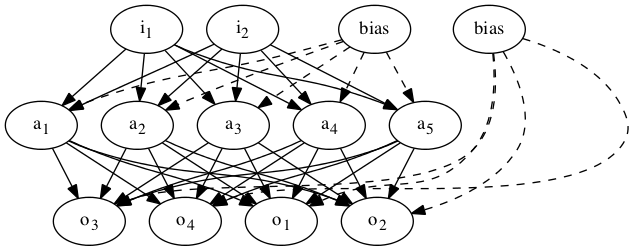
\includegraphics[width=300px]{1_net.png}

\subsection{Hypothesis}


When running both classifiers for a short time (i.e. 100 trees for the random forest and 100
epochs for the multi-layer perceptron) we expected the multi-layer perceptron to outperform the random forest.
This was because the multi-layer perceptron, by its nature, worked on continuous inputs while
the random forest needed to extrapolate discrete decision classes.

We expected the random forest to outperform the multi-layer perceptron after running a long
time (i.e. 10,000 trees or 10,000 epochs.) This was because the random forest was less likely to
overfit than the multi-layer perceptron.



\section{Data Sets}



Below are the sum of squared errors for the random forest solution and the multi-layer perceptron
solution. The random forest solution starts droping off at around 20\% while the
multi-layer perceptron drops off around 10\%. \\


{\center Random Forest} \\
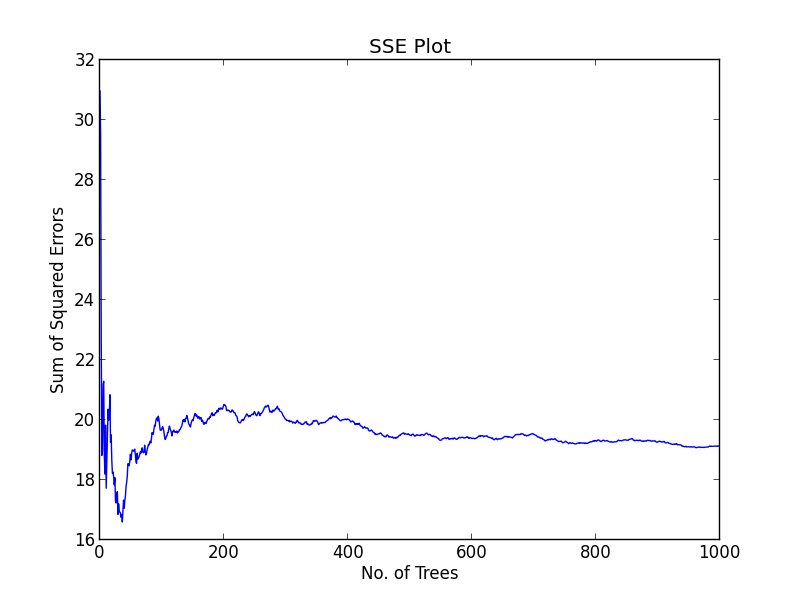
\includegraphics[width=200px]{dt_sse_training.png} \\


{\center Multi-layer Perceptron} \\
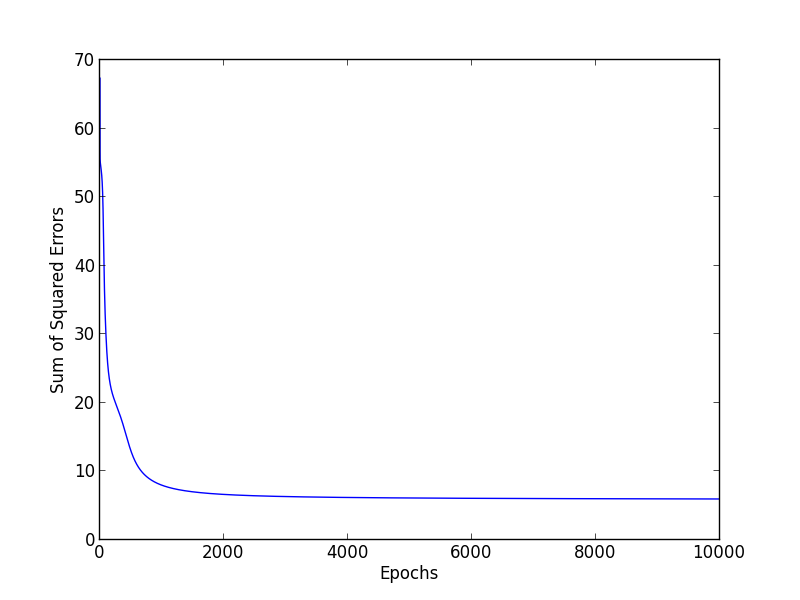
\includegraphics[width=200px]{mlp_sse_training.png}


\section{Results}


\subsection{Decision Tree Results}
\begin{tabular}{l l}
  Number of Trees &   Recognition Rate\\
  1               &   65\% \\
  10              &   95\% \\
  100             &   95\% \\
\end{tabular}

\subsection{Multi-layer Perceptron Results}


\begin{tabular} {l l }
  Number of Epochs & Recognition Rate \\
  1                & 30\% \\
  10               & 25\% \\
  100              & 55\% \\
  1000             & 100\% \\
\end{tabular}



\section{Discussion}
Our predections ended up being correct. The decision tree based random forest ended up
topping out at 95\% accuracy while the multi-layer perceptron had 100\% accuracy.

Interestingly enough, the random forest with 10 subtrees performed just as well as the one with 100
subtrees. This suggests that the 100-tree random forest might be overfit, and the 10-tree is good enough.
This seems even more true when you look at the error for the test data (section 2) and notice how the
error flattens well before 100 trees.




\end{document}
